\documentclass[12pt,aspectratio=169]{beamer}
% Set theme
\usetheme{metropolis}
% Place package includes Here
\usepackage{graphicx}
\usepackage{appendixnumberbeamer}
\usepackage{booktabs}
\usepackage{fontspec}
\defaultfontfeatures{Path=/Library/TeX/Root/texmf-dist/fonts/opentype/public/fontawesome/}
\usepackage{fontawesome}
\usepackage{pythontex}
\usepackage{svg}
% Title and author
\title{fiasco: a Python interface to the\\CHIANTI atomic database}
\subtitle{Heliophysics Community Python Working Group Meeting\\Boulder, CO USA}
\date{13 November 2018}
\author{Will Barnes}
\institute{Department of Physics and Astronomy, Rice University\\Houston, TX USA}
\titlegraphic{\hfill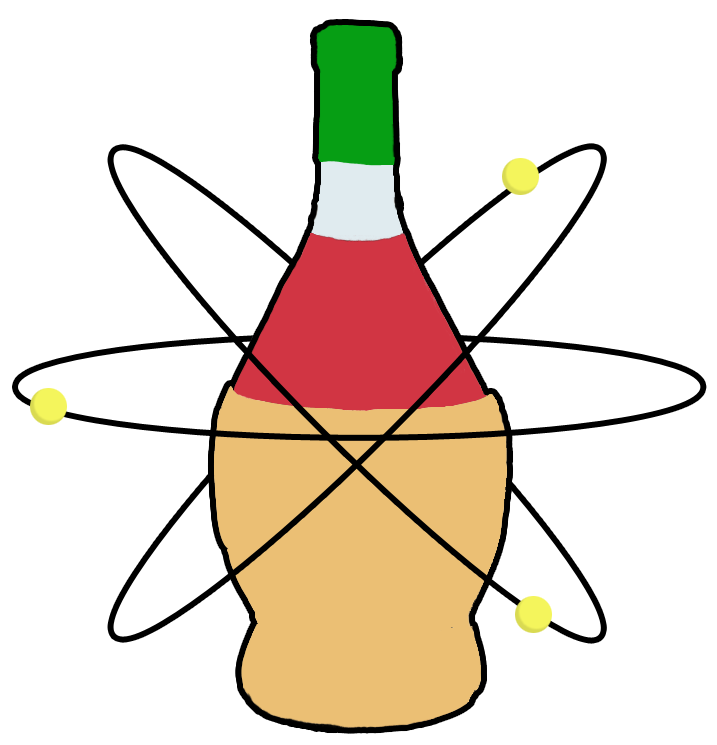
\includegraphics[height=1.5cm]{../figures/fiasco-logo.png}}

% Start Document
\begin{document}
% Title
\maketitle
% Contact
\begin{frame}{Contact Info}
    \begin{itemize}
        \LARGE
        \item[]\faicon{github} \texttt{wtbarnes}
        \item[]\faicon{twitter} \texttt{wtbarnes\_}
        \item[]\faicon{envelope} \texttt{wtb2@rice.edu} 
        \item[]\faicon{globe} \texttt{wtbarnes.github.io}  
    \end{itemize}
\end{frame}
% Content
\begin{frame}
    \begin{figure}
        \centering
        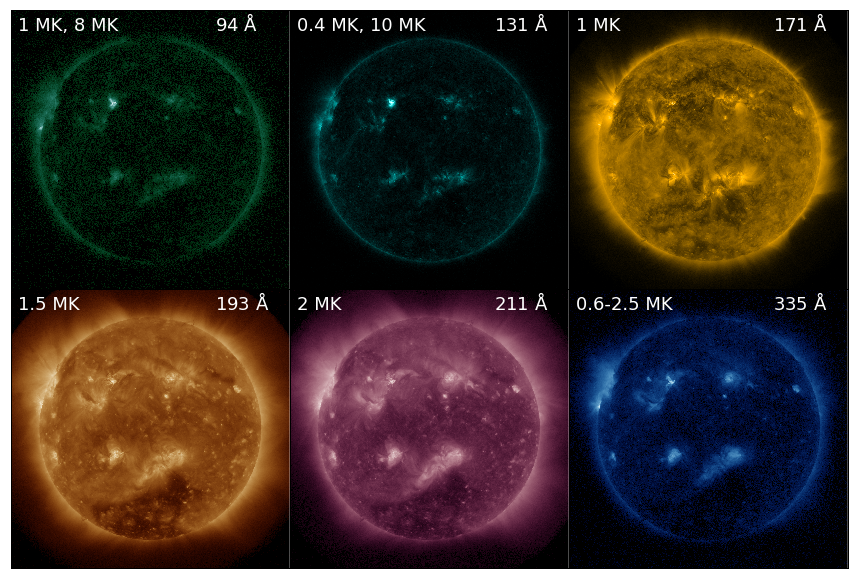
\includegraphics[width=0.9\textwidth]{../figures/aia_all_channels.png}
    \end{figure}
\end{frame}
%%%
\section{Parsing the Data}
%%
\begin{frame}[fragile]{Many Types of Files...}
    \scriptsize
    \begin{pygments}{bash}
        > tree ~/.fiasco/chianti_dbase/fe
            ├── fe_1
            │   └── fe_1.diparams
            ├── fe_10
            │   ├── fe_10.diparams
            │   ├── fe_10.drparams
            │   ├── fe_10.easplom
            │   ├── fe_10.easplups
            │   ├── fe_10.elvlc
            │   ├── fe_10.fblvl
            │   ├── fe_10.psplups
            │   ├── fe_10.rrparams
            │   ├── fe_10.scups
            │   ├── fe_10.wgfa
            │   └── fe_10_all.scups
            ...
    \end{pygments}    
\end{frame}
%%
\begin{frame}[fragile]{...in Many (Slightly) Different Formats}
    \tiny
    \begin{pygments}{bash}
> head -n 5 ~/.fiasco/chianti_dbase/fe/fe_10/fe_10.elvlc
1     3s2 3p5                           2  P    1.5          0.000          0.000
2     3s2 3p5                           2  P    0.5      15683.100      15683.000
3     3s 3p6                            2  S    0.5     289236.000     289236.000
4     3s2 3p4 3d                        4  D    2.5     388713.500     387464.000
5     3s2 3p4 3d                        4  D    3.5     388708.000     387566.000
    \end{pygments}
    \begin{pygments}{bash}
> head -n 6 ~/.fiasco/chianti_dbase/fe/fe_10/fe_10.scups
1      2   1.429e-01  -1.000e+00   1.940e-01   12    2   1.798e+01
0.000e+00   4.698e-02   1.097e-01   1.977e-01   3.302e-01   5.520e-01   7.114e-01   8.313e-01   9.249e-01   9.610e-01   9.801e-01   1.000e+00
6.022e+00   5.880e+00   5.690e+00   4.830e+00   3.790e+00   2.400e+00   1.530e+00   9.460e-01   5.190e-01   3.610e-01   2.790e-01   1.940e-01
1      3   2.636e+00   1.371e-01   2.080e-01   12    1   1.246e+00
0.000e+00   1.467e-01   2.949e-01   4.448e-01   5.971e-01   7.541e-01   8.300e-01   8.778e-01   9.149e-01   9.319e-01   9.435e-01   1.000e+00
1.024e+00   1.111e+00   1.198e+00   1.116e+00   9.116e-01   6.303e-01   4.751e-01   3.751e-01   3.030e-01   2.745e-01   2.572e-01   2.080e-01
    \end{pygments}
    \begin{pygments}{bash}
> head -n 10 ~/.fiasco/chianti_dbase/fe/fe_10/fe_10.drparams
1
26   10  2.0320e+03  1.0180e+04  4.6380e+04  1.6980e+05  4.4990e+05  7.8800e+05  0.0000e+00  0.0000e+00  0.0000e+00
26   10  5.3350e-04  1.8270e-03  4.8510e-03  2.7100e-02  8.2260e-02  3.1470e-01  0.0000e+00  0.0000e+00  0.0000e+00
-1
%file:  fe_10.drparams
%parameters for dielectronic recombination rate coefficients
Determined from the coefficients listed at:
http://amdpp.phys.strath.ac.uk/tamoc/DATA/RR/
These calculations have been performed by a collaboration of researchers at:
Auburn University, Rollins College, and the University of Strathclyde.
    \end{pygments}
\end{frame}
%%
\begin{frame}{Parser Factory}
    \begin{columns}
        \column{0.65\textwidth}
            \begin{itemize}
                \item Many filetypes with many "quirks"
                \item \texttt{ParserFactory} metaclass creates parser classes "on the fly"
                \item Filetype determines parser class using a \textit{factory pattern}
                \item In most simple case, parser class just provides
                \begin{itemize}
                    \item headings
                    \item units
                    \item types
                    \item descriptions
                \end{itemize}
            \end{itemize}
        \column{0.35\textwidth}
            \includegraphics[width=\columnwidth]{../figures/parser_inheritance_diagram.pdf}
    \end{columns}
\end{frame}
%%
\begin{frame}[fragile]{Parser Factory}
\footnotesize
\begin{pyconsole}
from fiasco.io import Parser
p = Parser('fe_16.elvlc')
p.parse()[:3]
type(p)
\end{pyconsole}
\end{frame}
\begin{frame}[fragile]{Parser Factory}
\scriptsize
\begin{pyconsole}
from fiasco.io import Parser
p = Parser('al_6.psplups')
p.parse()[:3]
type(p)
print(p.parse().meta['footer'])
\end{pyconsole}
\end{frame}
%%
\begin{frame}{Resources}
    \begin{itemize}
        \large
        \item[]\faicon{github} \texttt{wtbarnes/fiasco}
        \item[]\faicon{book} \texttt{fiasco.readthedocs.io}
        \item[]\faicon{code} \texttt{wtbarnes/heliopython-2018-talk}
        \item[]\faicon{globe} \texttt{chiantidatabase.org}   
    \end{itemize}
\end{frame}
\end{document}
